\chapter*{Task 2}
\addcontentsline{toc}{chapter}{Task 2}

Task 2 requires computing a smooth state-input curve. Then, it is required to compute the optimal trajectory as in Task 1.

We have designed the trajectory as a smooth transition between equilibrium points.

Since we have to impose the initial and final configurations and velocities for each joint, we need at least a third-order polynomial curve to transit from one equilibrium point to another.

For the first joint $q_1$, we impose the initial and final angles, both with zero velocity. The corresponding curve is defined as:


\begin{equation} \label{smooth_q1}
    \begin{aligned}
         &q_1(t) = a_0 + a_1t + a_2 t^2 + a_3 t^3 \\
         &\Dot{q_1}(t) = a_1 + 2a_2 t + 3a_3 t^2 \\
         &a_0 = q_{1i}\\
         &a_1 = 0\\
         &a_2 = 3 (q_{1f} - q_{1i})/(t_f^2)\\
         &a_3 = -2 (q_{1f} - q_{1i})/(t_f^3)
    \end{aligned}
\end{equation}

For the second joint $q_2$, we compute it as
\begin{equation} \label{smooth_q2}
    \begin{aligned}
            &q_2(t) = z - q_1(t) \quad z = 0 \lor \pi \\
            &\Dot{q}_2(t) = - \Dot{q}_1(t)
    \end{aligned}
\end{equation}

The value of $z$ is chosen depending on the configuration we want to maintain:

\begin{itemize}
    \item $z = \pi$, the second link is pointing upwards.
    \item $z = 0$, the second link is pointing downwards.
\end{itemize}

The input is computed as the gravity compensation along the smooth curve.

Once the reference has been computed, to improve the initial guess used to start the Newton's method algorithm, we try to track the reference with an LQR feedback computed on the linearization about it.

Since the trajectory is a sequence of equilibria, we get a solution for the LQR, only if the motions are quite slow. The reason is that if we try to track a quasi-static trajectory, since the second joint is not actuated, it is difficult for the control law to track the reference for fast motions.

Moreover, since the reference is not a true trajectory, the linearized dynamics is of the form:

\begin{equation}
\begin{aligned}
       &\Delta x_{t+1} = A_t \Delta x_t + B_t \Delta u_t + c_t \\
       & c_t = f(x^{ref}_t,u^{ref}_t) - x^{ref}_{t+1}
\end{aligned}    
\end{equation}

where the $c_t$ term is not zero.

In this case, we have chosen the same equilibrium points as before:

\begin{equation*}
\begin{aligned}
    &x_{init} = [0,0,0,0] \\
    &x_{fin} = [90,-90,0,0]
\end{aligned}  
\end{equation*}

A smooth reference transition has been chosen (Fig \ref{fig:downward_0_smooth}), and as it is possible to see, it is much easier to track than a step. The time of simulation is selected as 10 seconds, and the discretization time is 0.01 seconds.

The weights in the cost have been selected as before:

\begin{equation*}
    \begin{aligned}
        &Q_t = \begin{bmatrix}
            1000 & 0 & 0 & 0 \\
            0 & 1000 & 0 & 0 \\
            0 & 0 & 10 & 0\\
            0 & 0 & 0 & 10
        \end{bmatrix} = Q_T\\
        &\\
    & R_t = 10
    \end{aligned}
\end{equation*}

The algorithm takes 3 iterations to converge to a solution. As can be seen from the descent direction figure (\ref{fig:Downward_Descent_smooth}), the value of the norm goes below $10^{-6}$, which is the value we chose for the threshold.

\begin{figure}
    \centering
    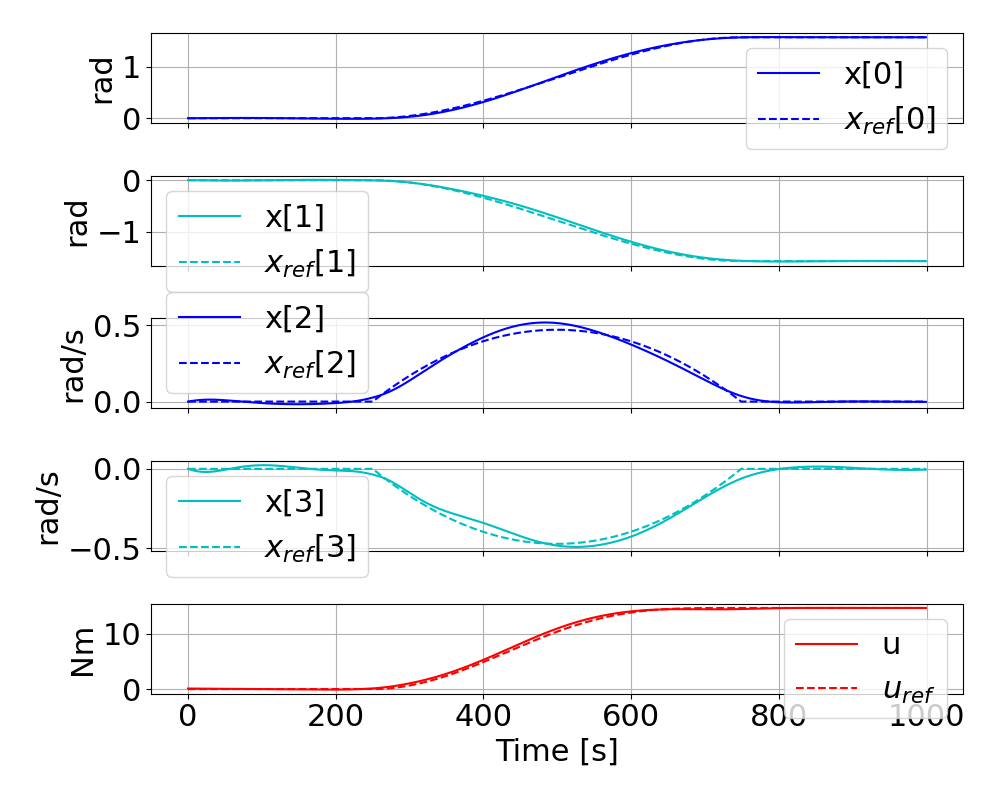
\includegraphics[width=0.8\linewidth]{figs/downward_0_smooth.png}
    \caption{Reference and initial guess}
    \label{fig:downward_0_smooth}
\end{figure}

\begin{figure}
    \centering
    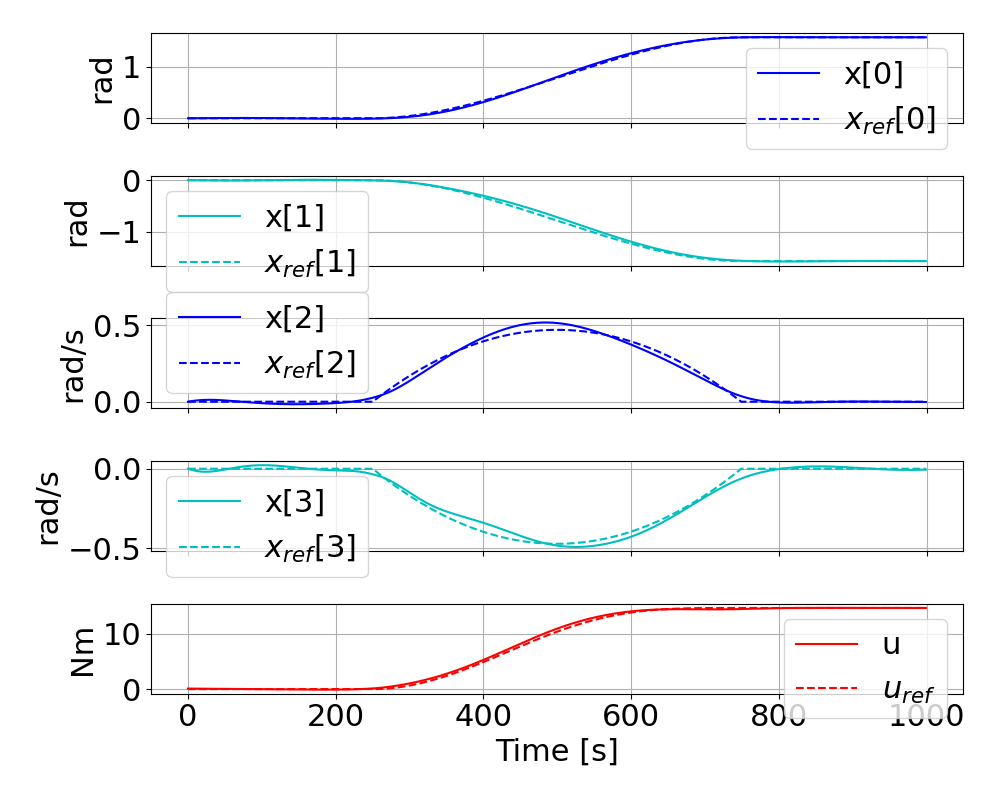
\includegraphics[width=0.8\linewidth]{figs/downward_1_smooth.png}
    \caption{First iteration}
    \label{fig:downward_1_smooth}
\end{figure}

\begin{figure}
    \centering
    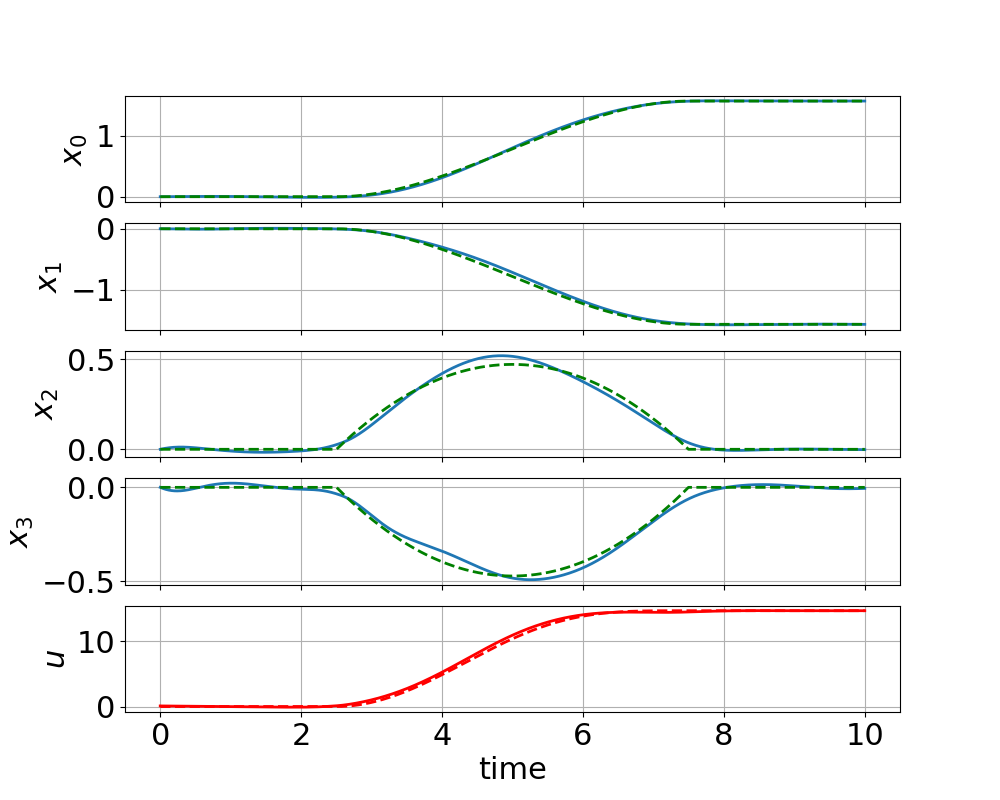
\includegraphics[width=0.8\linewidth]{figs/downward_f_smooth.png}
    \caption{Final result}
    \label{fig:downward_f_smooth}
\end{figure}

\begin{figure}
    \centering
    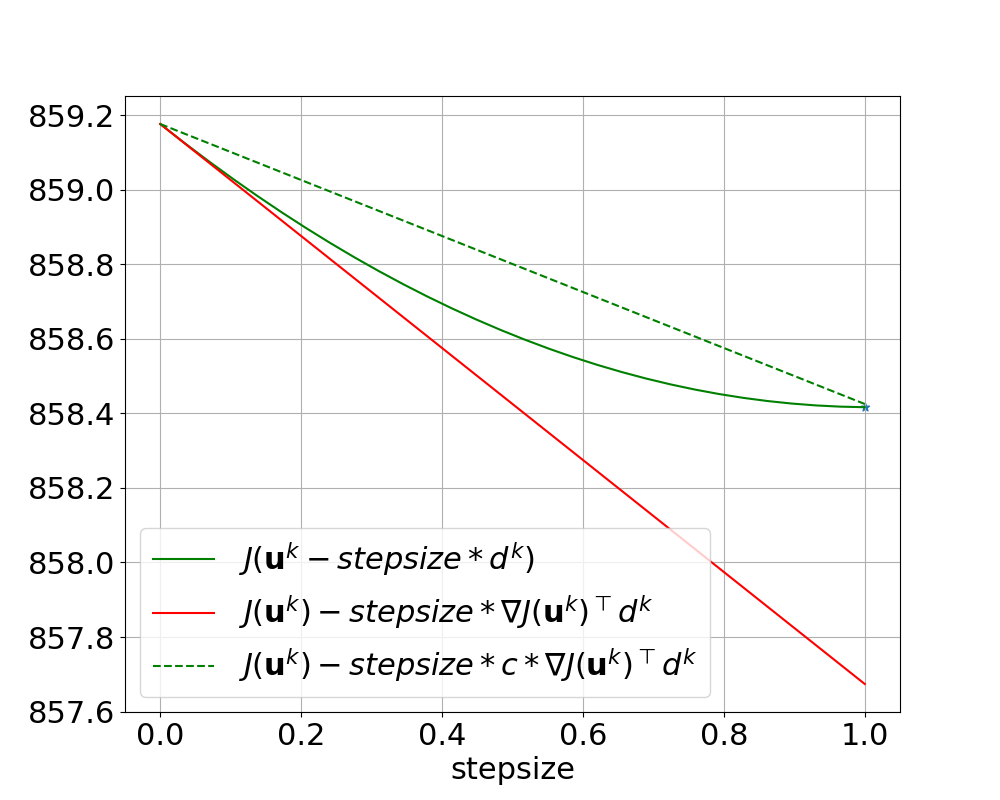
\includegraphics[width=0.8\linewidth]{figs/downward_armijio_0_smooth.png}
    \caption{Backtracking line search plot at the first iteration}
    \label{fig:downward_armijio_0_smooth}
\end{figure}

\begin{figure}
    \centering
    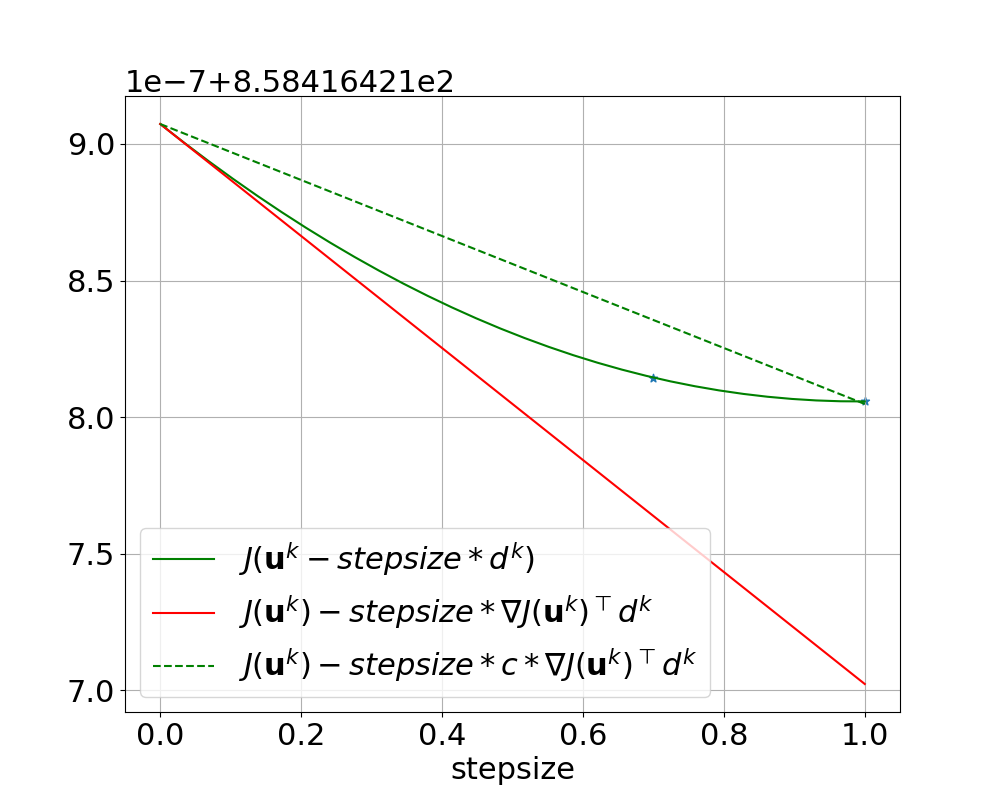
\includegraphics[width=0.8\linewidth]{figs/downward_armijio_f_smooth.png}
    \caption{Backtracking line search plot at the final iteration}
    \label{fig:downward_armijio_f_smooth}
\end{figure}

\begin{figure}
    \centering
    \begin{subfigure}[b]{0.49\textwidth}
        \centering
        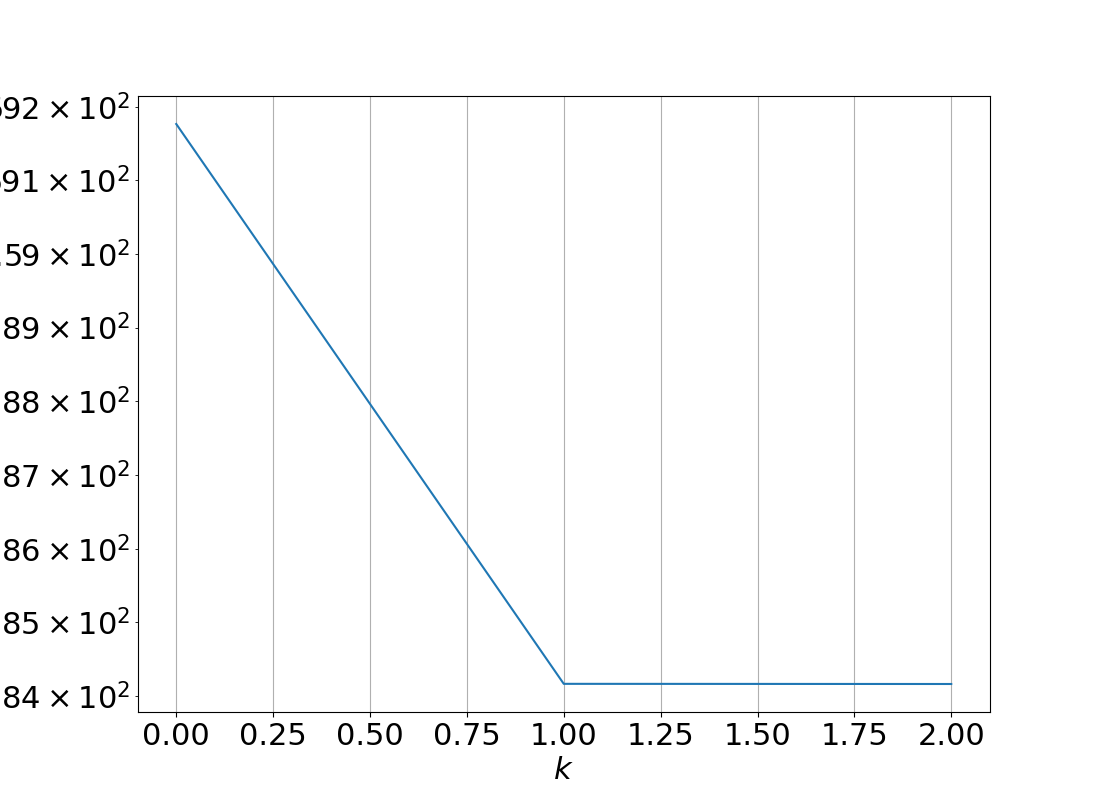
\includegraphics[width=\textwidth]{figs/downward_cost_smooth.png}
        \caption{Cost}
        \label{fig:downward_cost_smooth}
    \end{subfigure}
    \hfill
    \begin{subfigure}[b]{0.49\textwidth}
        \centering
        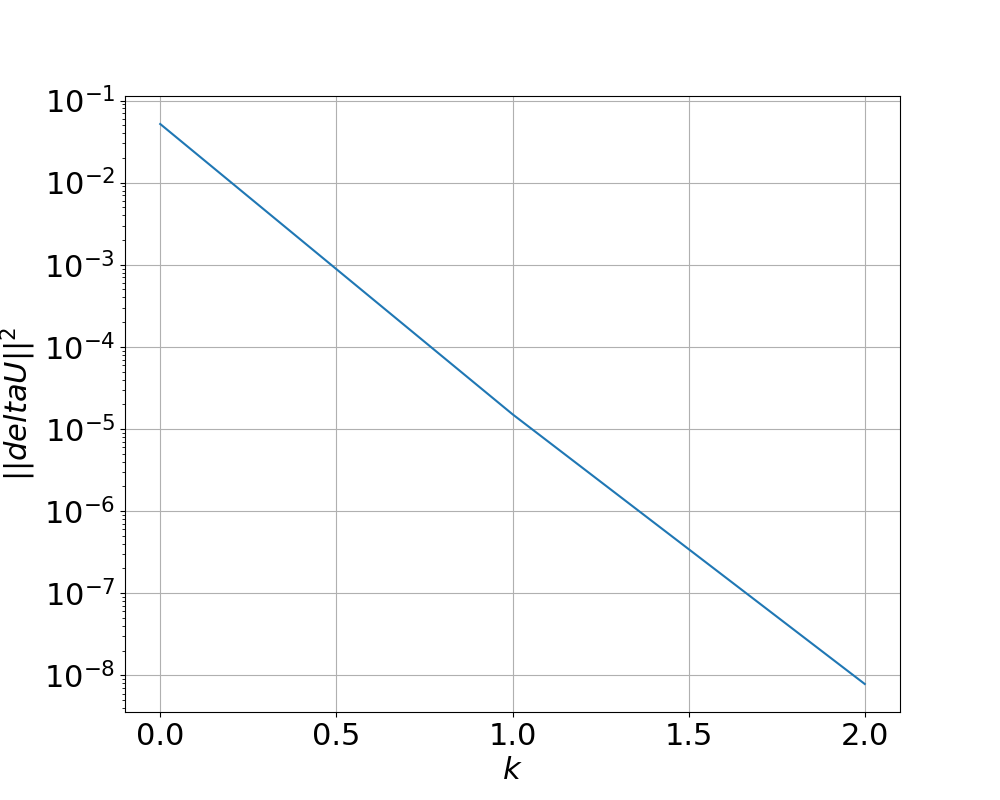
\includegraphics[width=\textwidth]{figs/Downward_Descent_smooth.png}
        \caption{Descent direction}
        \label{fig:Downward_Descent_smooth}
    \end{subfigure}
    \caption{}
\end{figure}

\section*{Python code}

The smooth reference trajectory has been defined in the python file reference\_trajectory.py. In the code several functions are defined:

\begin{itemize}
    \item \textbf{poly3(xx\_init, xx\_fin, tf, dt) }:Compute a smooth curve between xx\_init and xx\_fin connecting the two points with polynomial functions of order three. The input is computed as the gravity compensation along the obtained state reference curve. The initial and final configurations should be equilibrium points, and the reference curves are computed according to (\ref{smooth_q1}) and (\ref{smooth_q2}). The computation of $q_2$ depends on the given initial configuration. If the sum $q_1 + q_2$ at the initial configuration equals $0$, the equation for the upward arm is used. Conversely, if it equals $\pi$, the equation for the downward arm is used.  \\\\
    \textbf{Arguments}:
    \begin{itemize}
        \item xx\_init : Initial state vector in degrees.
        \item xx\_fin : Final state vector in degrees.
        \item tf : Final time in seconds.
        \item dt : Time of dicretization in seconds.
    \end{itemize}
    \textbf{Return}:
    \begin{itemize}
        \item xx\_ref : Reference curve between the two states from 0 to tf, in radiants.
        \item uu\_ref : Input reference curve.
    \end{itemize}
    
    \item \textbf{smooth\_comp(points, tf, dt) }: Compute a composition of smooth curve between state configuration points. The input is computed as the gravity compensation along the obtained state reference curve.\\\\
    \textbf{Arguments}:
    \begin{itemize}
        \item points : List of state vectors in degrees.
        \item tf : Final time in seconds.
        \item dt : Time of dicretization in second.
    \end{itemize}
    \textbf{Return}:
    \begin{itemize}
        \item xx\_ref : State reference curve in radiants.
        \item uu\_ref : Input reference curve.
    \end{itemize}

    \item \textbf{initial\_guess(xx\_ref, uu\_ref, tf, dt) }: Compute a state-input trajectory tracking the system about a smooth reference curve using an LQR solution implemented in the \textbf{LQR\_solver()} (see Task 3 for more details). \\\\
    \textbf{Arguments}:
    \begin{itemize}
        \item xx\_ref : Reference state vector.
        \item uu\_ref : Reference input vector.
        \item tf : Final time in seconds.
        \item dt : Time of dicretization in seconds.
    \end{itemize}
    \textbf{Return}:
    \begin{itemize}
        \item xx\_r : State trajectory.
        \item uu\_r : Input trajectory.
    \end{itemize}
\end{itemize}